\chapter{Mysteries and concluding remarks}
\label{wild}

\section{Extensive Air Showers}
\label{unusual}

Although built primarily for the detection of \gls{uhe} neutrinos, \gls{anita} is able to observe radio waves from \gls{eas} or \gls{cr} interactions in the air in a sideband channel. 
Neutrino candidates in \gls{anita} are expected to be primarily \gls{vpol}, while \gls{cr} candidates are primarily \gls{hpol}.
Interaction of the charged particles in the air with the local vertically upward-pointing geomagnetic field renders the radio signal from \gls{cr} candidates its \gls{hpol} signature. 
This is a fortunate difference between radio signal from neutrinos and that from cosmic rays. 

Although \gls{anita} has not yet discovered \gls{uhe} neutrinos, it has measured signal from several \gls{cr} candidates. There were 16 \gls{cr} candidates in the \gls{anita}-1 flight, a few in the \gls{anita}-2 flight and about 20 in the \gls{anita}-3 flight. Fewer \gls{cr} candidates were measured in the \gls{anita}-2 flight as the hardware was designed to not trigger on \gls{hpol} events in this flight. 

There are two ways in which \gls{anita} can measure the radio signature of \gls{eas}. These are 1) direct and 2) reflected as shown in a cartoon in Figure~\ref{eas_cartoon}. Radio waves due to \gls{cr} initiated particle showers in the air interacting with the local geomagnetic field can either reach the \gls{anita} payload directly as shown with a red line in the cartoon on the left side. Or, radio waves from the particle shower interaction with the geomagnetic field can reach the payload by reflection off of the ice as shown with two red lines in the cartoon on the right side.

\begin{figure}
\centering
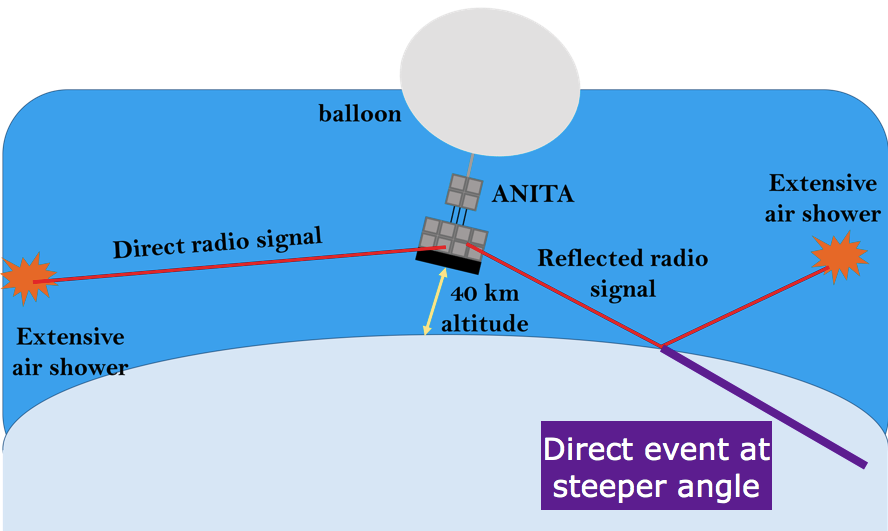
\includegraphics[width=1.0\textwidth]{figures/anita_cartoon_me.png}
\caption{Cartoon explaining how ANITA observes extensive air showers. Red lines denote the paths of radio waves from extensive air showers interacting with the geomagnetic field reaching the ANITA payload. The purple line indicates the implicated trajectory of the mystery events.}
\label{eas_cartoon}
\end{figure}

\subsection{Unusual upgoing events}

We have reported on the observation of two unusual, upgoing events~\cite{me1,me2}. They are referred to as mystery event 1 and 2, respectively. They were both \gls{eas} candidates. Mystery event 1 is from the \gls{anita}-1 flight and mystery event 2 is from the \gls{anita}-3 flight. They were both found to be \gls{hpol} events and \gls{cr}-like. 

Whether \gls{anita} observed an event directly or by reflection can be determined from the polarity of the event waveform. 
Typically, \gls{anita} measures \gls{cr} events as reflected events whose polarity is opposite to that of directly observed events.  The two mystery events had polarity consistent with that of being directly observed events. The polarity of mystery event 2 can be seen in Figure~\ref{polarity_me2}. Here the field strength in mV per meter is in the vertical axis and time is in the horizontal axis. A dip or trough in the waveform can be seen. This trough would be a peak for an event of opposite polarity. 

It can be seen from Figure~\ref{eas_cartoon} that directly observed \gls{eas} events in \gls{anita} have shallower elevation angles than those observed by reflection off of the ice. Directly observed \gls{cr} events are relatively rare and usually observed at shallow angles of a few degrees below the horizontal. Both mystery events 1 and 2 have steeper elevation angles of $-27.4^{\circ}$ and $-35^{\circ}$, respectively. These elevation angles are typical of reflected events, not direct. This is shown with a purple line on the right side of the cartoon in Figure~\ref{eas_cartoon}. 

To summarize, the mystery events had polarity consistent with being direct events but elevation angles similar to that of reflected events.
The unusualness of the two mystery events lie in the incompatibility between their observed polarity and the elevation angle at which they were seen.
We elaborate further by summarizing the publication on mystery event 1 in Section~\ref{summary_me1}. 


\subsection{Detailed summary of Mystery Event 1}
\label{summary_me1}

I summarize here the publication on Mystery Event 1~\cite{me1}. 
In this publication, we reported on four \gls{cr} or \gls{cr}-like events observed with \gls{anita}. From \gls{anita}’s first flight in 2007, 16 \gls{uhecr} air showers were reported, 13 of which were consistent with geomagnetically-induced radio pulses seen in reflection off the Antarctic ice surface. Three of these 16 events in the signal box (expected background was 1.6 events) from the initial blind analysis were deemed background: two of unknown origin and one a likely thermal noise fluctuation with no apparent signal content. Three additional CRs were also found in cross-correlation analysis after unblinding including two events that were identified as Earth-skimming \gls{cr}s, a previously unobserved class of events. The Earth-skimming events were directly observed and thus had opposite polarity as the reflected events. In addition to these two Earth-skimming events observed in \gls{anita}-1, another event of the same type was observed in \gls{anita}-2. 

\begin{figure}
\centering
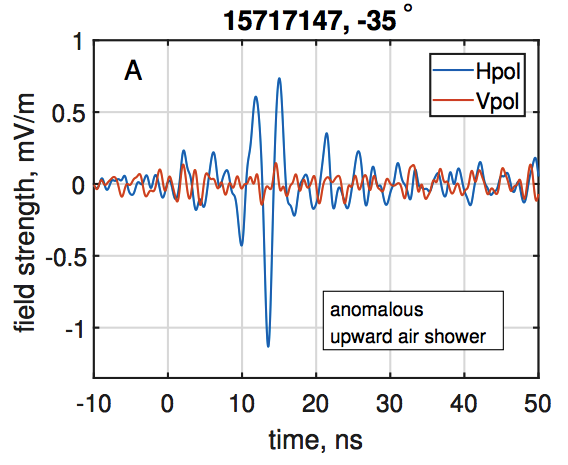
\includegraphics[width=0.8\textwidth]{figures/polarity.png}
\caption{Figure from ANITA publication on mystery event 2~\cite{me2}. This shows the polarity of mystery event 2. 
The trough seen in the waveform would be a peak for a reflected event.}
\label{polarity_me2}
\end{figure}

On reviewing the events in the signal box of \gls{anita}-1, it was found that one of the events, previously deemed background, was dominated by \gls{hpol} content and consistent with geomagnetic parameters of a \gls{cr}. It arrived at the payload from a direction of $27.4^{\circ}$ below the horizontal, a fairly typical angle for a reflected \gls{cr} event. Interestingly, however, it did not correlate well with a reflected \gls{cr} signal shape. A re-evaluation of this event led to the finding that the polarity of this event is consistent with an air shower seen directly, without reflection. Naturally, then, this event was compared to the other class of \gls{cr}s, the Earth-skimming events. But the three Earth-skimming \gls{cr} events showed in~\cite{me1} have much shallower angles associated with them, namely, 4.3, 3.3 and 3.0 degrees below horizontal. So, the steep angle of $27.4^{\circ}$ below horizontal of this \gls{cr}-like event poses interesting problems for interpretation. 

The publication~\cite{me1} investigates these four unusual upward-directed events seen by ANITA with the goal of explaining what relation, if any, these may have with tau lepton initiated air showers. In case any of these events are associated with tau leptons, then an exciting interpretation would be that the tau lepton originated from the charged current interaction of a UHE tau neutrino in the ice or, more likely, in the rock below the ice, and then survived long enough to produce a directly (as opposed to reflected) observed air shower.

A radio signal detected by ANITA can have a mix of polarization states, that is, it can be part unpolarized, part linearly polarized and part circularly polarized. Stokes parameters I, Q, U and V can be estimated for signals to figure out the different polarization components of a signal. The I parameter is for unpolarized, Q is for linearly polarized (+Q for Hpol and –Q for Vpol), U is for linearly polarized along 45 degrees (+U for positive slope, -U for negative slope) and V is for circularly polarized (+V for left circularly polarized and –V for right circularly polarized).

In case of \gls{cr}s, at least a few percent of circular polarization may be expected in the signal due to possible interference between the primary geomagnetic radiation and secondary Cherenkov radiation. Upon estimating the Stokes parameters for the four events in~\cite{me1}, it was found that in addition to linear polarization, the two stronger Earth-skimming events have circular polarization components. The \gls{cr}-like mystery event, too, has both linear and circular polarization (~ 10\%) components. The presence of circular polarization, the good correlation with the other three upward-directed \gls{cr} events and with the inverted reflected \gls{cr} events, excess of noise in trailing part of the signal similar to reflected \gls{cr}s, all support that the \gls{cr}-like mystery event originates primarily from geomagnetically-induced radiation. 

The two competing hypotheses about the \gls{cr}-like mystery event are as follows: it could be a reflected \gls{cr} event whose polarity got distorted by some unknown process OR it could be a direct air shower event caused by interactions or decay of a secondary lepton from a neutrino interaction in the Earth. The most probable candidate for a secondary lepton in the latter hypothesis is a tau lepton. After accounting for uncertainties, the minimum possible emergence angle for the hypothesized tau event is 25.4 degrees below horizontal which corresponds to an Earth chord distance of 5460 km. This chord distance is about 17,000 km water equivalent which is far greater than the Standard Model (SM) predicted neutrino interaction length of about 2000 km water equivalent. A neutrino with energy of order EeV or more with Standard Model cross section would not make it far enough through this Earth chord to produce a tau lepton late enough for the tau to then survive long enough to produce an air shower. 

Since the energies of the events are known to be of order EeV or more from the observed radio pulses, the only other parameter that can be tweaked to consider the tau hypothesis is the cross section. It is found that for SM cross sections of the neutrino, more events closer to the horizon should have been seen. When the cross section is suppressed, however, ANITA’s acceptance (prediction for the number of neutrinos expected to be seen by ANITA, call it apples) for such events agree with current limits (call it oranges) with the caveat that the limits are all derived using SM cross sections (cannot compare apples to oranges). However, it is interesting to see that suppressing the cross section by a factor of about 3-5, as initially estimated in~\cite{me1},
does make the \gls{cr}-like mystery event present itself reasonably as a tau neutrino candidate. 


\section{Investigating the mystery events}

Mystery event 2 was found at the same time as when we were completing a search for a diffuse flux of \gls{uhe} neutrinos in data from the third flight of \gls{anita}. Event 15717147 or mystery event 2 was cut in the binned analysis by the elevation angle cut. If forced to pass this cut, it was still removed by the CPol peak strength cut. 

To look at where mystery event 2 reconstructed on the continent compared to other events from the \gls{anita}-3 flight, I made the plot shown in Figure~\ref{me_map}. Here most points are blue and denote the reconstructed location of events from the \gls{anita}-3 flight that have passed all but a final set of cuts. The satellite stripe cut has also been applied to these events. 

The solid red dots in Figure~\ref{me_map} denote the locations to which mystery event 1 and 2 were reconstructed on the continent. Note that we show mystery event 1 here although this event is from the \gls{anita}-1 flight. A solid red cross is also shown near each red dot. These denote the location of the \gls{anita} payload at the time of recording the corresponding mystery event. It can be seen that for both mystery events, the ANITA payload is located {\bf above} the red dot, that is, above the reconstructed location of the mystery event. It could have been that one red dot was below the corresponding red cross, and the other red dot above the corresponding red cross.  But that does not happen. From this, it is conceivable that there is a ``source" in the direction towards the bottom of this plot that \gls{anita} is ``facing" during the time of recording both mystery event 1 and 2. 

\subsection{Satellite influence}

A possible source that \gls{anita} could be facing during the time of recording the mystery events is a satellite or group of satellites. It should be noted that the latitude of the \gls{anita} payload is about $-82^{\circ}$ both during mystery event 1 and mystery event 2. Therefore, during both mystery events, \gls{anita} was able to view the {\bf same} satellites because which satellites come into view depend on the latitude of the observer. The two mystery events were plotted using red dots overlaid on the satellite stripe plot as shown in Figure~\ref{me_stripe}. They are labeled in white as ``ME1" and ``ME2". In black dots are shown the events that passed all but a clustering cut in the binned analysis of the \gls{anita}-2 flight. 

Both mystery events can be seen to lie on the same central stripe in the satellite stripe plot in Figure~\ref{me_stripe}. Although in this figure the central stripe shows up as faded in the middle, this is not a plot that shows the stripes as a function of time. At the time of recording mystery event 1, \gls{anita} was at the same latitude as during recording mystery event 2 and was able to see the same satellite or group of satellites that is represented by the central stripe. Both mystery events lying on the same satellite stripe is consistent with \gls{anita} viewing the same satellite or group of satellites during both.

\begin{figure}
\centering
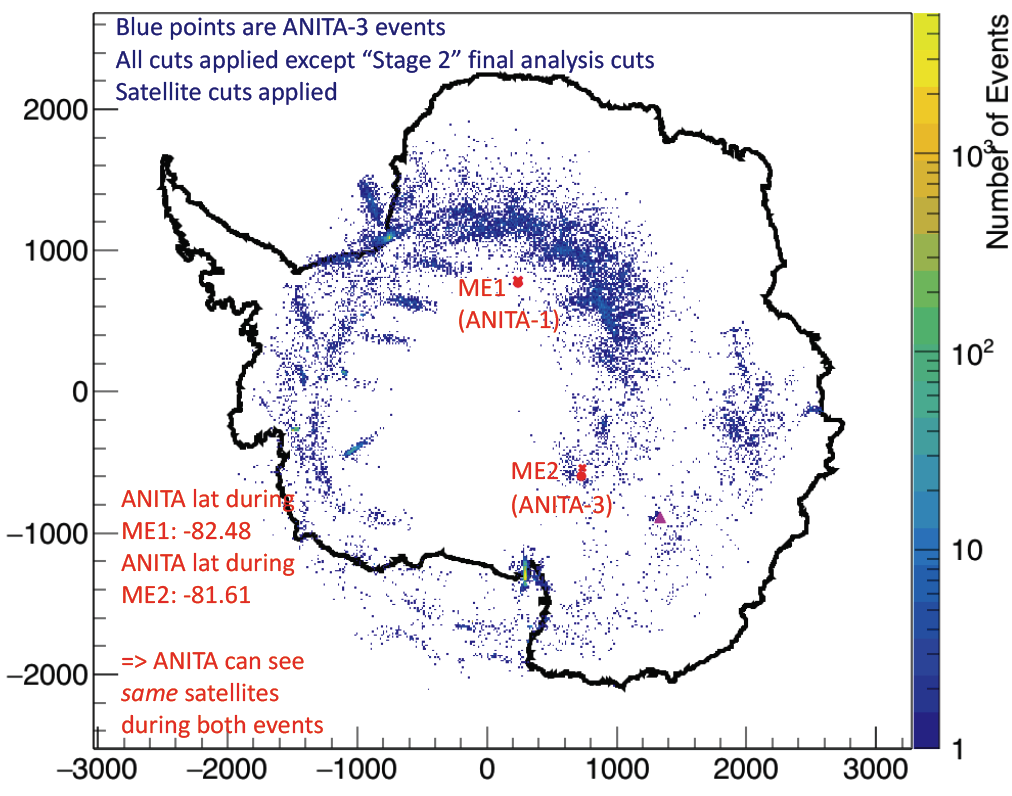
\includegraphics[width=0.8\textwidth]{figures/me_map.png}
\caption{Map showing events (blue points) from the ANITA-3 flight before final cuts. Overlaid are positions of the mystery events 1 and 2, labeled here as ME1 and ME2. Note that the latitude of  the ANITA payload during both mystery events is about $-82^{\circ}$. The same satellites are viewable by the ANITA payload during both events.}   
\label{me_map}
\end{figure}

So were the mystery events somehow caused by satellites? We are not yet sure about this. As is evident from~\cite{me1,me2}, both mystery events were impulsive in nature. Such a signature is not expected to come from satellites. Satellites have been known to cause modulated \gls{cw} noise, not impulsive events. 

In addition to being impulsive, the mystery events were isolated and passed the clustering cuts of the clustering analyses. 
Could \gls{cw} interference from satellites influence impulsive events from bases in Antarctica to reconstruct elsewhere, for example, as mystery events? This is something we started to investigate. We looked at events from the three different passes of the \gls{anita} payload over Bin 3045 of the \gls{anita}-2 binned analysis. The three passes of the payload are shown in Figure~\ref{bin3045_3passes}. 

We plotted the events from each pass as shown in Figure~\ref{pass1} and \ref{pass3}. Here the elevation angle of event reconstruction is plotted in the vertical axis, the azimuth angle in the horizontal axis and the color represents the number of events. Figure~\ref{pass1} shows events from the first pass of the payload over Bin 3045. Figure~\ref{pass3} shows events from the third pass of the payload over Bin 3045. It can be seen that the reconstruction of events on the left is much better in the first pass than in the third pass. Assuming the events on the left are due to a base of human activity on the continent, the non-alignment of the base with a satellite during the first pass could be the reason why the reconstruction is tighter here.
We hypothesized that when a satellite or group of satellites is {\bf aligned} with a ground pulse in azimuth, it could cause events from the ground pulse to reconstruct less tightly. In other words, an event that should have reconstructed to a base could be influenced by satellites to reconstruct elsewhere and {\bf appear} isolated. Whether satellites do have this effect or not needs to be further studied and quantified. 


\begin{figure}
\centering
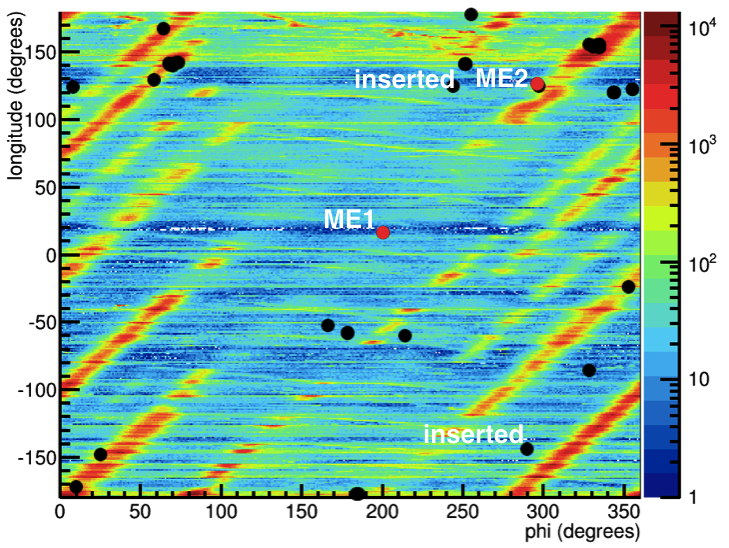
\includegraphics[width=0.8\textwidth]{figures/me_stripe.png}
\caption{Mystery events 1 and 2 overlaid on the satellite stripe plot using solid red markers. The solid black indicate events that passed in the ANITA-2 binned analysis.}
\label{me_stripe}
\end{figure}


\begin{figure}
\centering
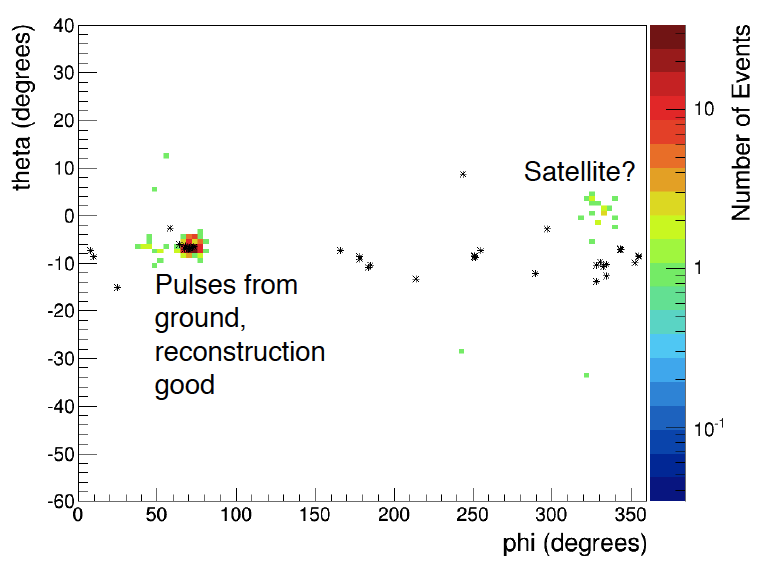
\includegraphics[width=0.8\textwidth]{figures/bin3045_pass1.png}
\caption{Events from pass 1 of the ANITA payload over Bin 3045 of the ANITA-2 binned analysis.}
\label{pass1}
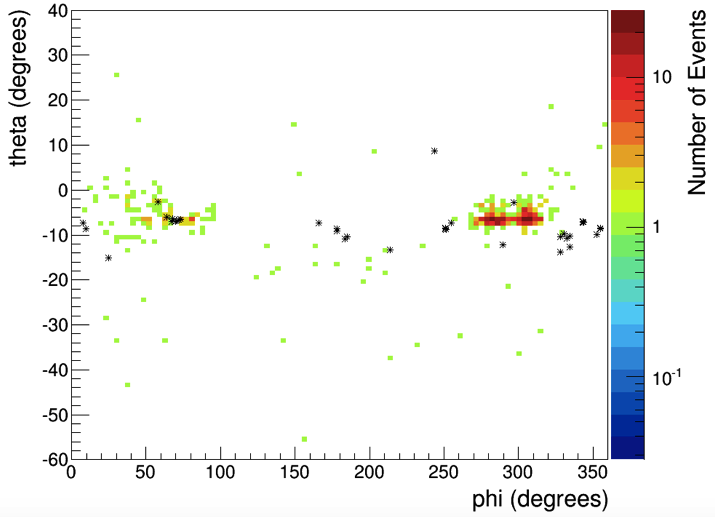
\includegraphics[width=0.8\textwidth]{figures/bin3045_pass3.png}
\caption{Events from pass 3 of the ANITA payload over Bin 3045 of the ANITA-2 binned analysis. This is the pass from which five excess events passed in this analysis. }
\label{pass3}
\end{figure}


\section{Simulating reduced cross sections}

To investigate the effect of cross section on observable polarization angle, we simulated neutrinos of different energies and cross sections using icemc. 
We did this for three different energies: $10^{18}\,\mbox{eV}$, $10^{19}\,\mbox{eV}$ and $10^{20}\,\mbox{eV}$), and five different cross sections: \gls{sm} cross section, \gls{sm} cross section times 0.3, 0.1, 0.03, and 0.01. 
We tested this with the \gls{anita}-2 simulation because it is well-tested but we selected events that triggered in both LCP and RCP to remove any V/H bias. 
This had come up in discussions about designing the \gls{anita}-4 trigger, and when discussing the mystery event 1. 

We made distributions of the plane-of-polarization angle with respect to the vertically polarized E-plane and calculated the corresponding cumulative distribution functions. We also made two-dimensional distributions of the \gls{vpol} E-plane and \gls{hpol} E-plane. These are shown in Figures~\ref{polangle20}, \ref{polangle20_cdf} and \ref{sm_2d}.
As can be seen in Figure~\ref{polangle20}, the polarization component along the VPol E-plane is negative if the signal is coming from the bottom of the Cherenkov cone leading to direction of polarization being anti-parallel to the VPol 
E-plane. 
The vertical axis of the CDF in Figure~\ref{polangle20_cdf} show the probability of getting a corresponding value or less in the horizontal axis. 

For \gls{sm} cross section, events tend to be close to vertical as expected (for Earth-skimming geometry) and for reduced cross sections we can see more of the Cherenkov cone which leads to a broader range of polarizations being observable. As can be seen in Figure~\ref{sm_2d}, the options for observable polarization angles increase dramatically when the cross section is reduced from \gls{sm} to 0.01 times \gls{sm}. Similarly, in Figure~\ref{polangle20}, the distributions of polarization angles become flatter and flatter with reduced cross section. 
We verified that for a VPol-based trigger there is even more of a bias for vertically polarized events. 


\begin{figure}
\centering
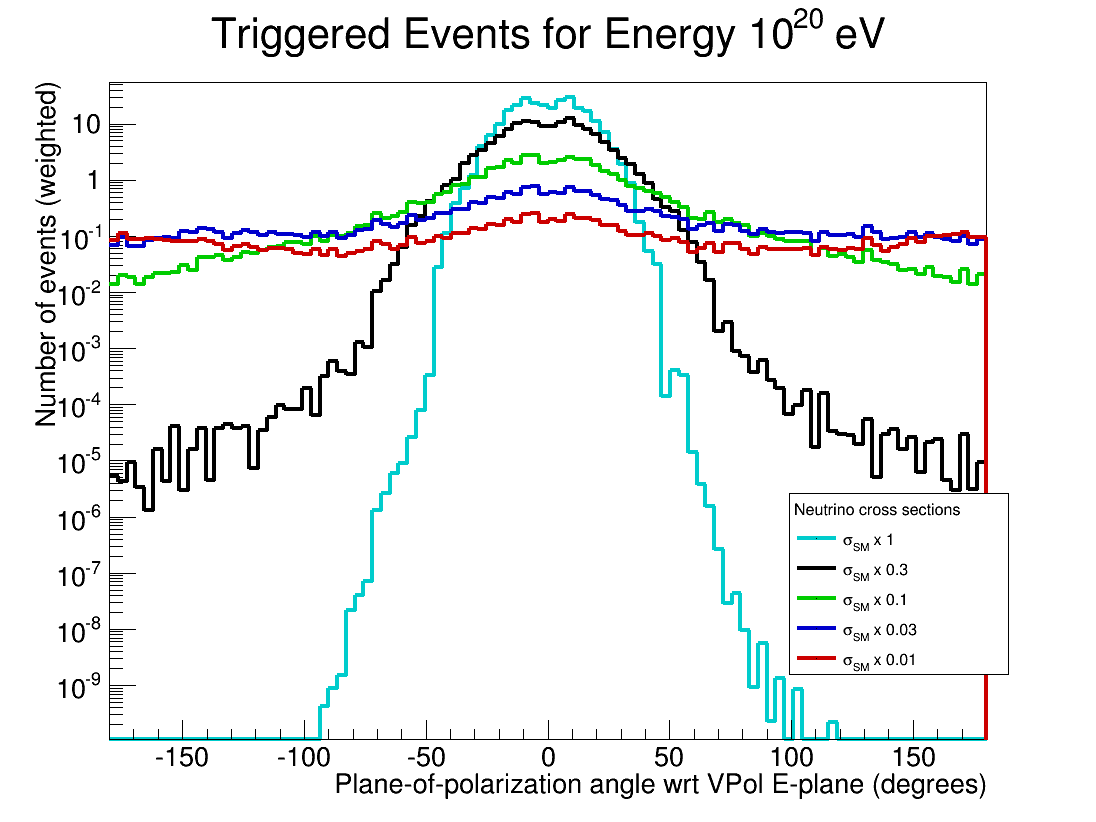
\includegraphics[width=0.8\textwidth]{figures/Balloon_polangle20.png}
\caption{Distribution of the plane-of-polarization angle wrt vertically polarized E-plane of simulated neutrino events of energy $10^{20}\,\mbox{eV}$ for different cross sections.}
\label{polangle20}
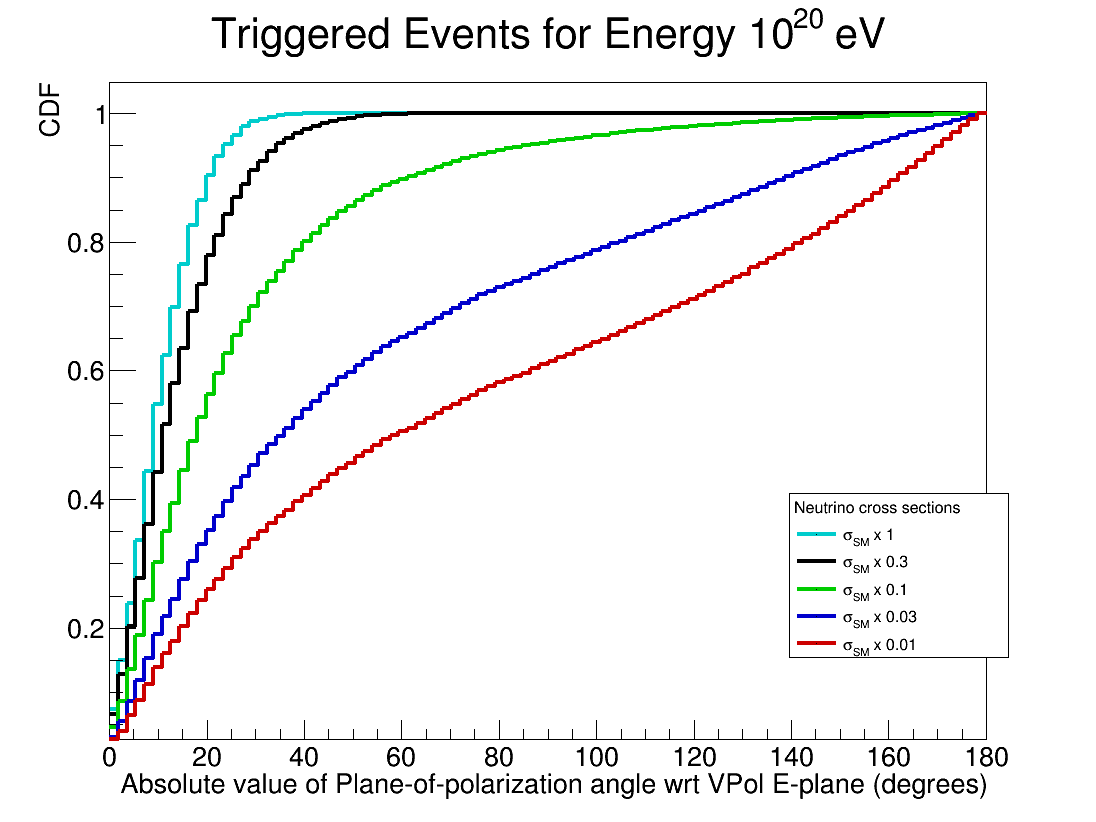
\includegraphics[width=0.8\textwidth]{figures/Balloon_cdf_polangle20.png}
\caption{CDF of the above distributions.}
\label{polangle20_cdf}
\end{figure}


\begin{figure}
\centering
\subfloat[SM x 1]{
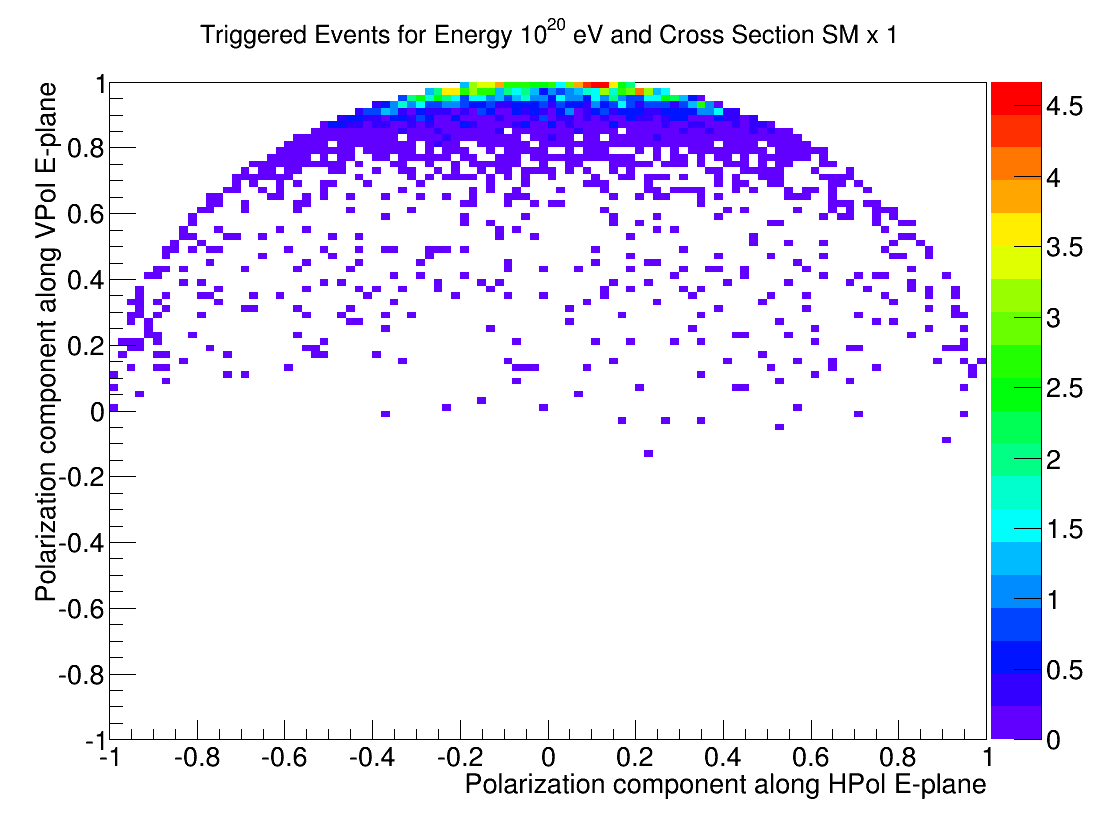
\includegraphics[width=0.5\textwidth]{figures/Balloon_2decomphcomp_cross1_20.png}
}\par 
\subfloat[SM x 0.3]{
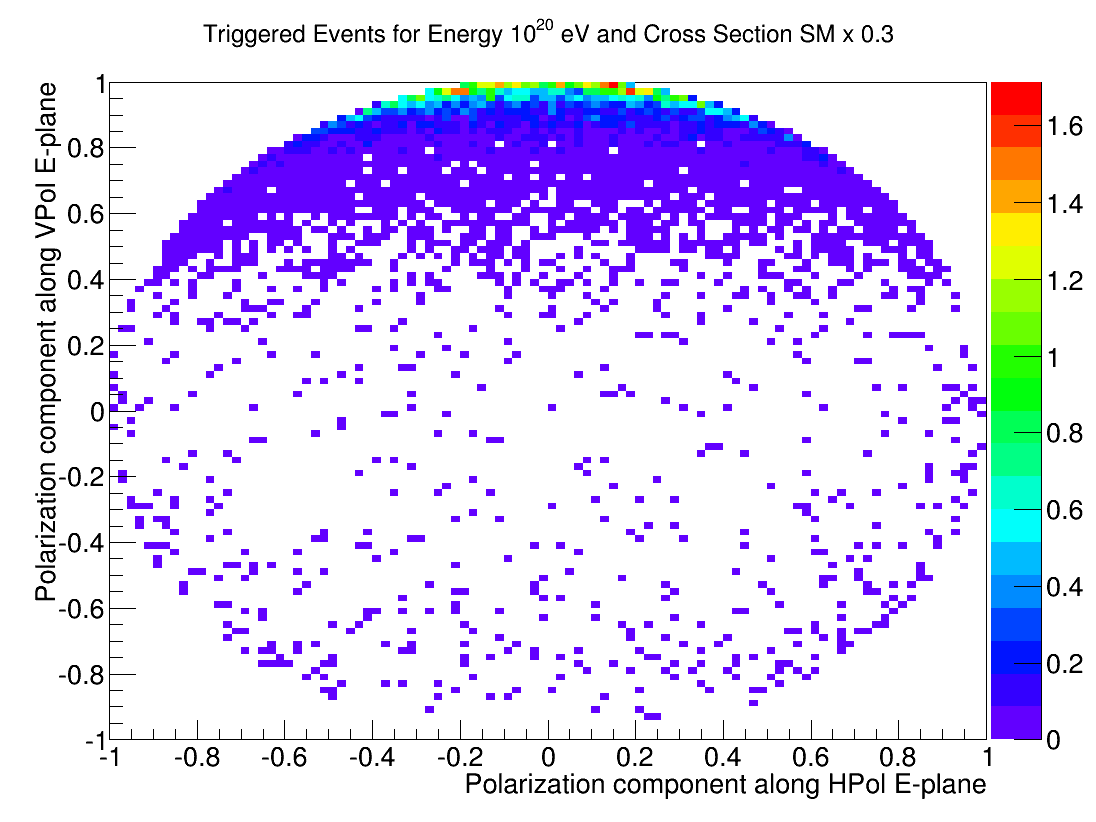
\includegraphics[width=0.5\textwidth]{figures/Balloon_2decomphcomp_cross0_3_20.png}
} \par 
\subfloat[SM x 0.01]{
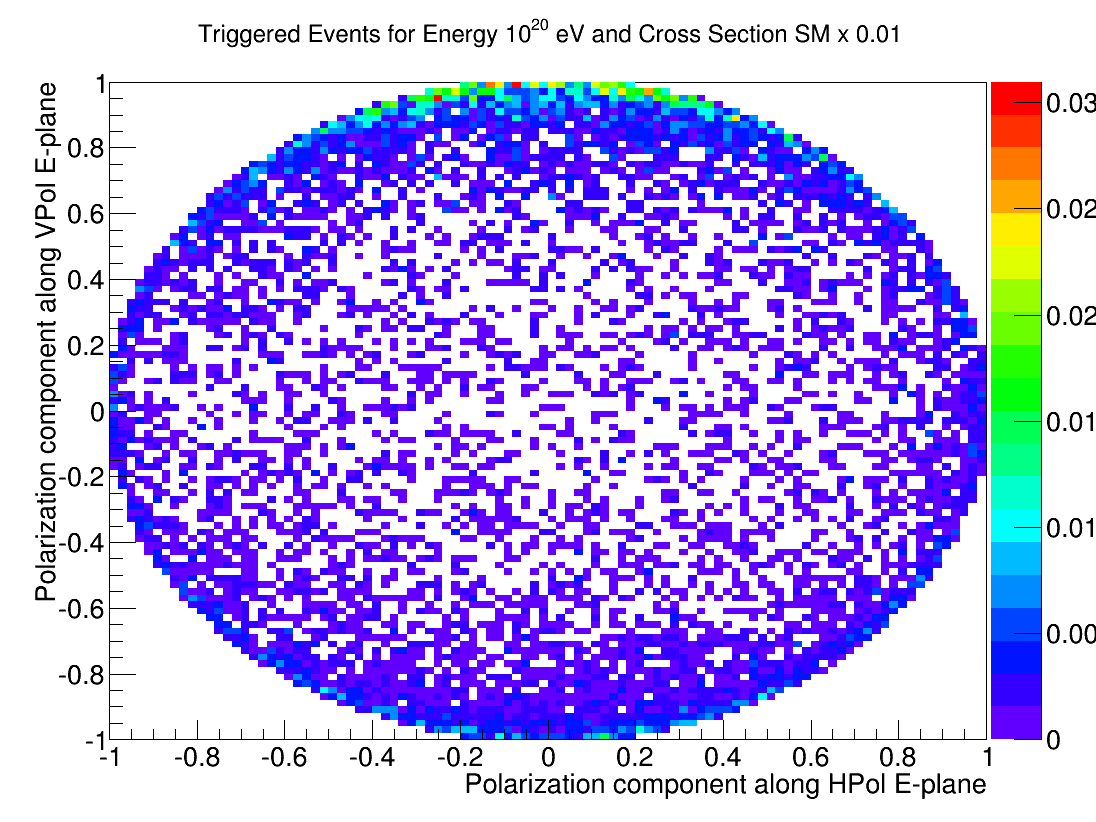
\includegraphics[width=0.5\textwidth]{figures/Balloon_2decomphcomp_cross0_01_20.png}
}
\caption{Two dimensional distribution of the polarization component along the vertically polarized E-plane in the vertical axis and that along the horizontally polarized E-plane along the horizontal axis. Color denotes the number of simulated, triggered neutrino events of energy $10^{20}\,\mbox{eV}$ and cross section 1, 0.3 and 0.01 times the Standard Model cross section in the top, middle and bottom plots, respectively.}
\label{sm_2d}
\end{figure}

\section{ANITA as a potential long-lived SUSY particle detector}
\label{susy}

We investigated the potential of \gls{anita} as a detector of long-lived, charged supersymmetric particles, such as staus. We propose that a stau could be detected by \gls{anita} through measurement of the \gls{eas} from the secondary tau, as a directly incoming, horizontally-polarized signal.
As explained in Section~\ref{unusual}, \gls{eas} signals recorded with elevation angles steeper than $6.5^{\circ}$ below the horizontal are typically ones that are reflected off of the ice, obtaining an opposite polarity. Thus, the non-inversion of the polarity of the recorded signal could be utilized to indicate their association with a stau.

We simulated the production of a stau inside the earth. It undergoes energy loss as it travels through the earth and then decays near the surface of the earth to create a tau. The tau also undergoes energy loss, leaves the earth and produces an air shower. This air shower, depending on geometry, could be observed by \gls{anita}. 

Figure~\ref{stau_plots} shows plots from this simulation. The top figure shows a two-dimensional distribution of stau masses and lifetimes. The color axis shows the probability of detection by \gls{anita} corresponding to a particular set of stau mass and lifetime. The elevation angle used here is $6.5^{\circ}$. It can be seen that parts of the parameter space in mass and lifetime are more likely to be detectable than others. The bottom plot shows the 
differential probability of decay of a heavy, charged particle as a function of distance along its path through the earth. This is shown for four different combinations of stau masses and lifetimes. 

The probability of the tau decaying in air is calculated as an integral which takes the form below. Here, the assumption is that the primary neutrino produces a stau in the earth which after traveling inside the earth produces a tau inside the earth close to the surface of the earth. The tau then pops out of the earth and produces an air shower. 

\begin{equation*}
P = exp( \frac{-(C - D_{stau} + (d_{air} - d_{shower}))}{d_{tau}}
- exp( \frac{-(C - D_{stau} + d_{air})}{d_{tau}}
\label{stau_integral}
\end{equation*}

In the above equation, P is the probability of the tau decaying in air such that ANITA can view the resulting air shower.
C is the total earth chord length traveled by neutrino-stau-tau. This is given purely by geometry utilizing the elevation angle, which is $35^{\circ}$ for the second unusual upgoing event. 
The quantity $D_{stau}$ is the distance traveled by the stau inside the earth before decaying to a tau. This is based on the stau mass and lifetime. We try this for several combinations of stau mass and lifetime as shown in Figure~\ref{stau_plots}.
$d_{air}$ is the distance traveled by the tau shower in the air. This is based on geometry given that ANITA sees the shower.
$d_{shower}$ is the maximum distance away at which ANITA can start to see the shower. 
$d_{tau}$ is the distance traveled by the tau before it decays. The shower energy is assumed to be half of the tau energy.

Although intended as mainly an investigation of \gls{anita}'s potential as a detector of long-lived, charged particles, this study also serves as 
an investigation of the mystery events and whether they can be explained by physics involving staus. 
From our simulations, we found that, although it is possible to detect a stau at an elevation angle of $35^{\circ}$ for a particular set of stau mass and lifetime, it is more likely to detect stau signatures at shallower angles such as $6.5^{\circ}$. In other words, steeper angles may be possible but are not favored. The challenges of detecting this signature at steeper angles could be alleviated by the presence of a source sending bursts of \gls{uhe} neutrinos in a particular direction. Such a possibility could be further investigated in future. We remain optimistic, however, that \gls{anita} could serve as a detector of radio signatures of supersymmetric particles for complementary portions of the parameter space which cannot be probed by other experiments. 

\begin{figure}
\centering
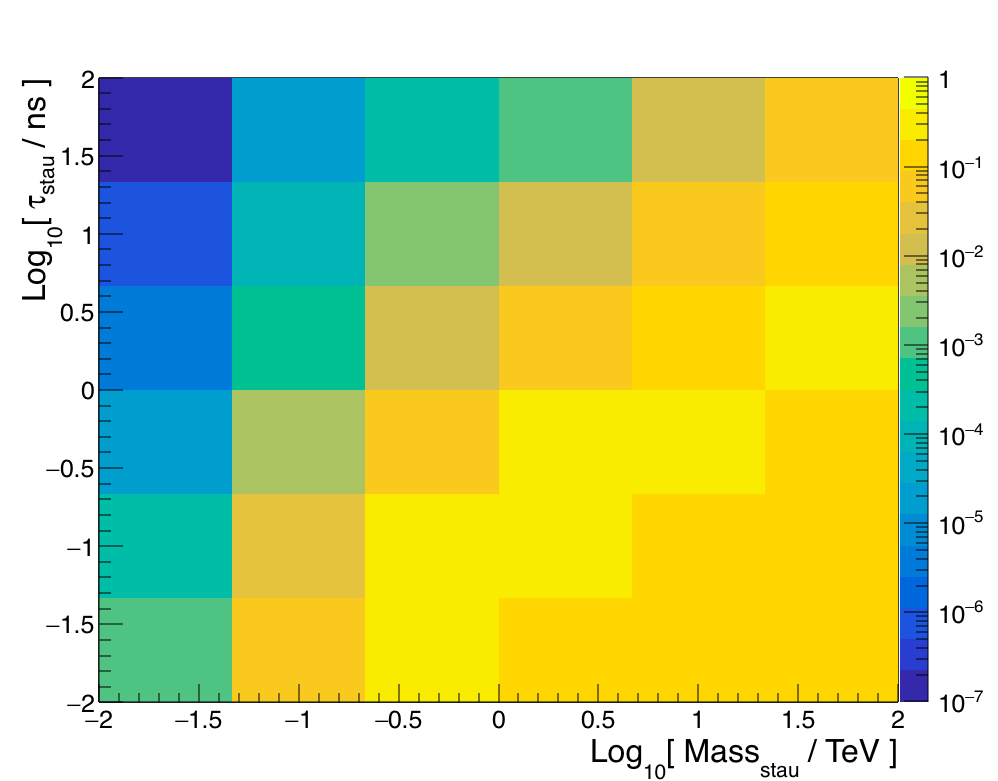
\includegraphics[width=0.8\textwidth]{figures/6_forthesis.png}
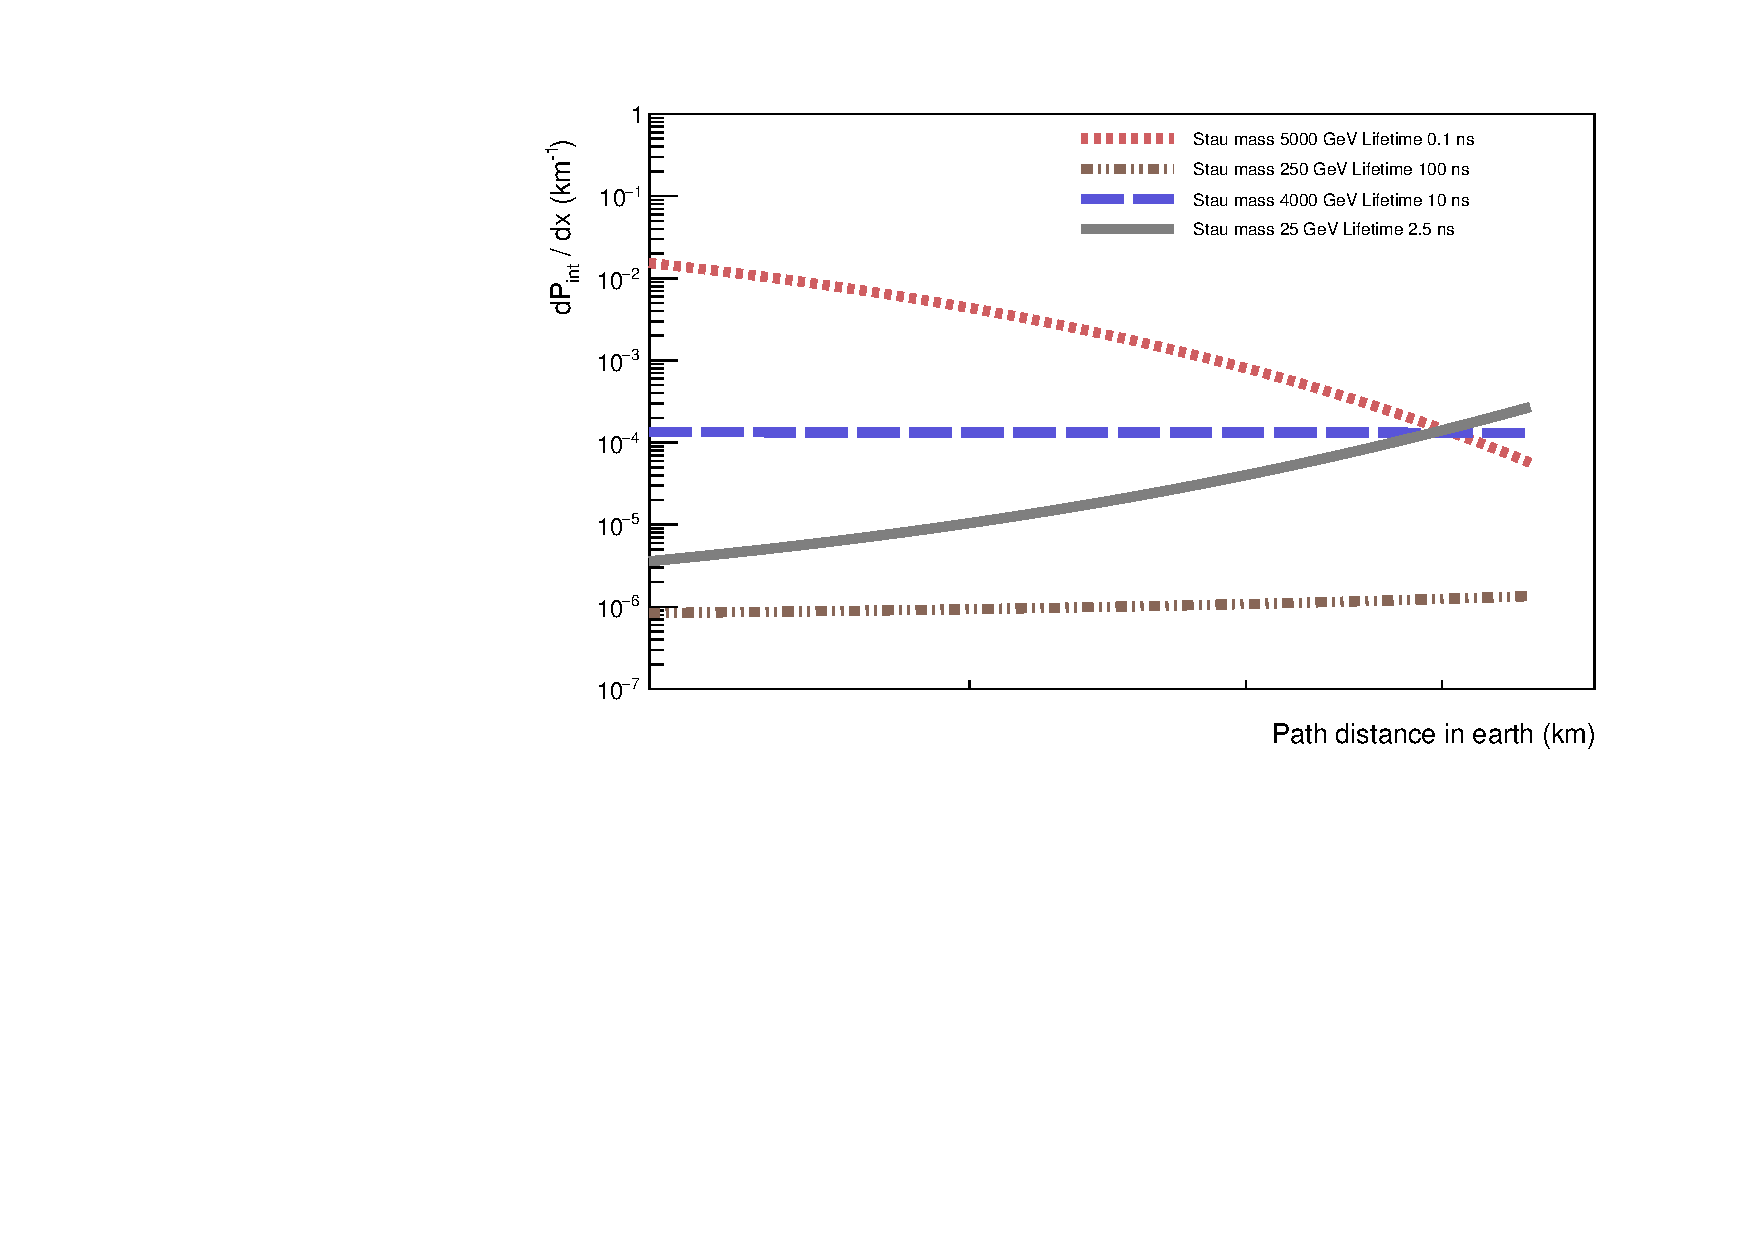
\includegraphics[width=0.8\textwidth]{figures/bragg_like_thesis.pdf}
\caption{Top: Distribution of stau mass and lifetime with color indicating the probability of detection. Bottom: Differential probability of decay of a heavy, charged particle as a function of distance along its path through the earth.  Different 
combinations of lifetimes and masses highlight different shapes that this can take.}
\label{stau_plots}
\end{figure}


\section{Conclusions}

It is an exciting time for particle astrophysics.
There have been major developments in the radio detection of \gls{uhe} neutrinos and extensive air showers. \gls{anita} has made two observations of potential \gls{uhe} tau neutrino candidates for the first time. It has been found that \gls{anita} also has the potential to be sensitive to exotic physics involving supersymmetric particles. 

The search for a diffuse flux of \gls{uhe} neutrinos in data from the third flight of \gls{anita} has been completed. A new limit has been placed on the diffuse flux of \gls{uhe} neutrinos. Around 25 \gls{eas} candidates were also discovered in the \gls{anita}-3 data, two of which were only discovered in the new binned analysis presented in this thesis. This thesis is also the first document to describe the details of the binned analysis results published for the first time in~\cite{diffuse}. The binned analysis has also been successfully extended to perform a search for neutrinos from \gls{grbs} with progress made in the development of the first search constrained in time as well as direction.

Lastly, the total instrument livetime of \gls{anita} has been tripled in \gls{anita}-4 by the \gls{tuff} notch filters. Details on these filters and associated results along with the first descriptions of the \gls{anita}-3 and -4 instruments are also part of this thesis and an associated publication~\cite{tuff}. This has paved the way for a much more (about 4 times more) sensitive instrument and the potential for further confirmation of ground-breaking observations as well as for new discoveries in particle astrophysics. 